% !TEX program = pdflatex
\documentclass[a4paper,11pt]{article}

\usepackage{geometry}
\usepackage{graphicx}
\usepackage{siunitx}
\usepackage{amsmath}
\usepackage{amssymb}
\usepackage{enumerate}
\usepackage{multirow}
\usepackage{floatrow}
\usepackage{xcolor}
% !TEX root = ../a2.tex
\usepackage{minted}
\usepackage{listings}
\usepackage{xcolor}
\usepackage{caption}
% \usemintedstyle{monokai}
\definecolor{bg}{rgb}{0.95,0.95,0.95}

\newcommand{\inputcode}[4]{
    \begin{longlisting}
        \caption{#3}
        \inputminted[xleftmargin=25pt, linenos, breaklines, bgcolor=bg]{#1}{#2}
        \label{#4}
\end{longlisting}}
\newenvironment{longlisting}{\captionsetup{type=listing}}{}

\geometry{top=0.8in, bottom=1.3in, left=0.8in, right=0.8in}

\newcommand{\e}[1]{\times10^{#1}}
\newcommand{\degree}{^\circ}
\newcommand{\spl}[1]{\[\begin{split}{#1}\end{split}\]}
\newcommand{\enum}[1]{\begin{enumerate}[(1)]{#1}\end{enumerate}}
\newcommand{\dd}{\text{d}}
\newcommand{\LA}{\Leftarrow}
\newcommand{\RA}{\Rightarrow}
\newcommand{\LR}{\Leftrightarrow}
\newcommand{\m}{\backslash}
\renewcommand{\listingscaption}{Program code}

\linespread{1.3}

\begin{document}

% !TEX root = ../a2.tex
\newcommand{\HRule}{\rule{\linewidth}{0.5mm}}
{
\center

\HRule \\[0.4cm]
\textsc{\huge VE281 Homework II}\\[0.4cm]
{\Large\textbf{Performance Analysis for Selection Algorithms}}\\[0.4cm]
{\large \textbf{Name:} Tianyi  \textsc{Ge}\quad \textbf{Stu Number:} 516370910168}\\[0.2cm]
\HRule \\[1.5cm]
}
% !TEX root = ../a1.tex

\section{Introduction}
In this report, we discuss the time complexity of six types of different sort algorithms including Bubble sort, Insertion sort, Selection sort, Merge sort and two types of Quick sorts, by testing their average runtime with input in different sizes.  The graph of time-size relationship, intuitively demonstrates the time complexity, thus confirming our theoretical expectation.

Furthermore, this report entails several extreme situations like an integer array in descending order or an array of merely 1's. The result, interestingly, reflects the capacity of those six algorithms under different circumstances.

Since the time complexity of $O(n^2)$ and $O(n\log n)$ differs enormously with the increasing of input size, we separate the analysis into two parts and discuss respectively.

\section{Performance analysis on $O(n^2)$ Sort Algorithms}
\begin{figure}[H]
    \centering
    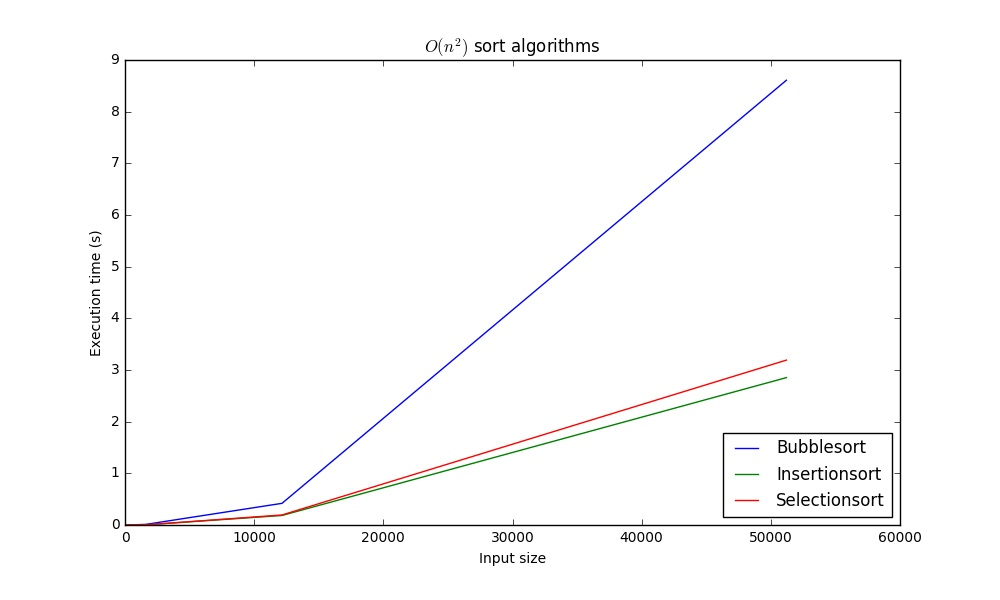
\includegraphics[width=0.8\linewidth]{../a1/012}
    \caption{Performance of $O(n^2)$ sort algorithms}\label{012}
\end{figure}
In Fig. \ref{012}, the curves are in shape of quadratic functions, among which the Bubble sort obtains a obvious larger constant. The runtime is considerably increasing non-linearly after the input size exceeds 25000.

\section{Performance analysis on $O(n\log n)$ Sort Algorithms}
\begin{figure}[H]
    \centering
    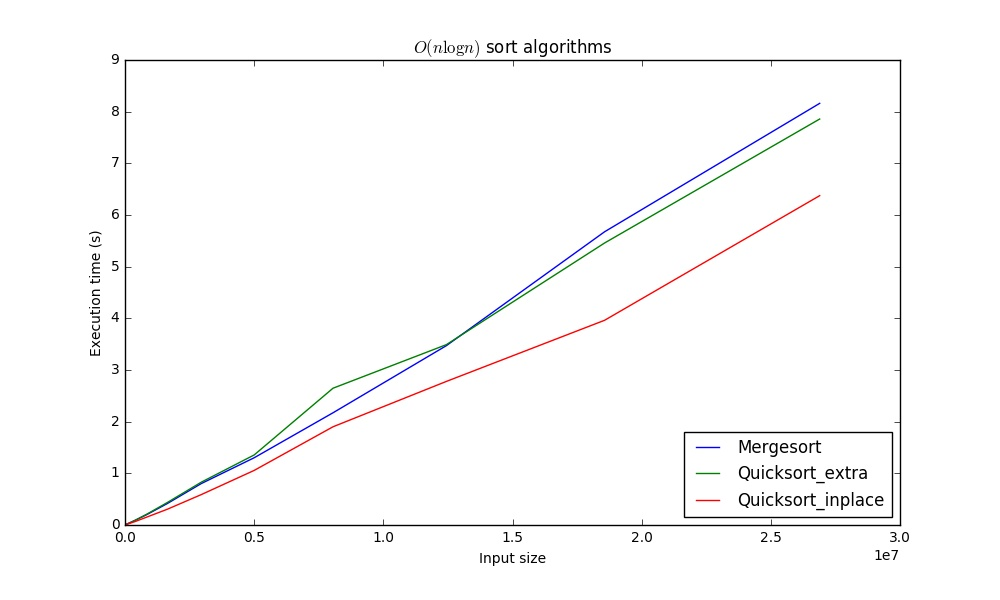
\includegraphics[width=0.8\linewidth]{../a1/345}
    \caption{Performance of $O(n\log n)$ sort algorithms}\label{345}
\end{figure}
In Fig. \ref{345}, the curves are almost linear, where the in-place Quick sort shows an undebatable edge. It's hard to tell whether it's $O(n\log n)$ or $O(n)$ because the input size is not large enough to give credit to the expectation. The distinction between two different Quick sort is intriguing. They followed almost the same procedure whereas a big gap occurred when even the input data is random. It shows that allocating memory is considerably time-consuming. This reflects It also indicates that the randomized Quick sort works remarkably, even compared to other steady $O(n\log n)$ algorithms like Merge sort.

\section{Extreme Input Situations}
\subsection{An Array in Descending Order}
For descending data, we still separate them into two categories. We observed that all of them become more efficient. One possible explanation is that the descending data guarantees that each element differs. Elements with the same value probably lead to slowing down.

In addition, the gap between Bubble sort and the other two $O(n^2)$ algorithms is shrinking, saying that their times of swap are approaching. In general, the complexities essentially follows their average performance. Quick sort does not degenerate back to $O(n^2)$.
\begin{figure}[H]
    \centering
    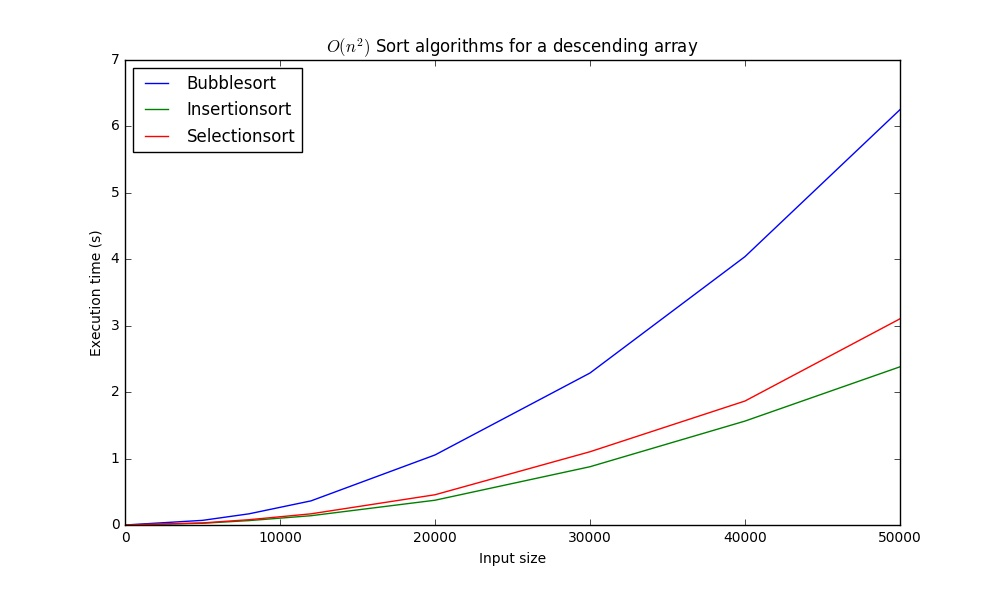
\includegraphics[width=0.8\linewidth]{../a1/reverse012}
    \caption{Performance of $O(n^2)$ sort algorithms}\label{r012}
\end{figure}
\begin{figure}[H]
    \centering
    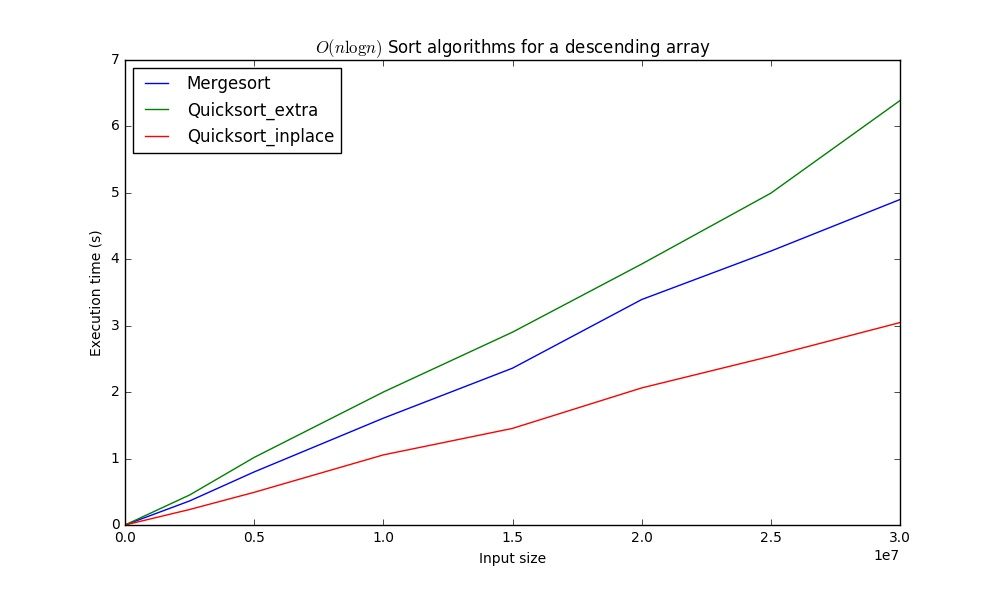
\includegraphics[width=0.8\linewidth]{../a1/reverse345}
    \caption{Performance of $O(n\log n)$ sort algorithms}\label{r345}
\end{figure}

\subsection{An Array of 1's}
\begin{figure}[H]
    \centering
    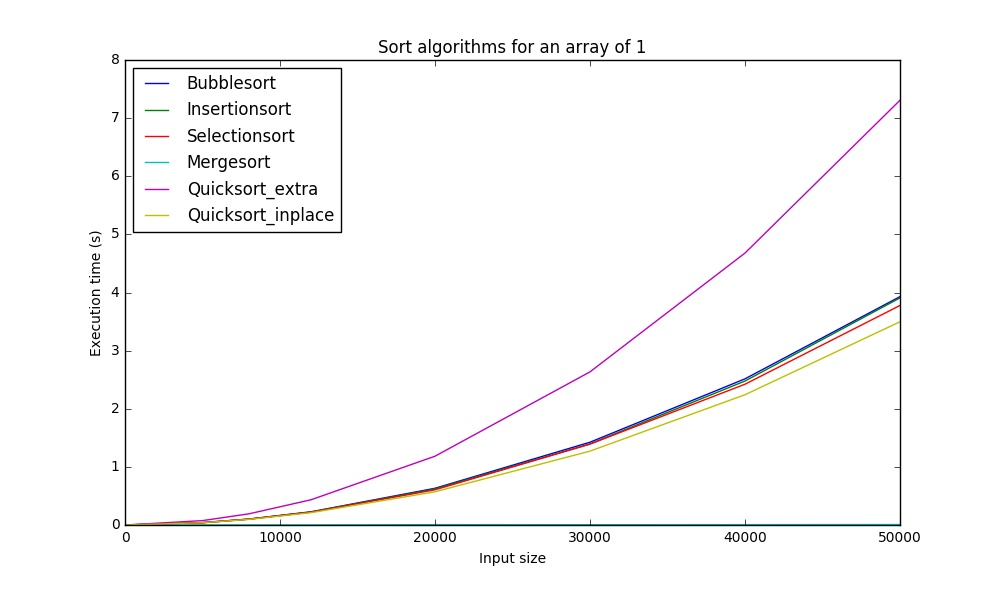
\includegraphics[width=0.8\linewidth]{../a1/same}
    \caption{Performance of $O(n\log n)$ sort algorithms in 1's array}\label{s}
\end{figure}
For this manipulated input, the performance of Quick sort precipitously degenerates, especially the version that requires extra space. Not only does it degenerate to $O(n^2)$ but also obtains a huge constant, even larger than Bubble sort. This phenomenon, again, indicates the flaw of frequently allocating memories.

On the contrary, Merge sort is quite steady. Whether the input is manipulated or not does not provoke a notable change on its performance, even though in average case it's still slower than in-place Quick sort.

\section{Conclusion}
In this report, we have demonstrated the characteristics of six different sort algorithms as well as their performance when the input is descending or all the same. Quick sort with extra memory is especially unsteady whose performance greatly depends on the input pattern. While the Merge sort, on the contrary, is brilliant on steadiness.

Also, the Insertion sort implemented with linked-list is an interesting case. It avoids $O(n)$ time to move the sorted part but involves extra memory allocation. Since $O(n^2)$ sort algorithms are not practicable in reality, here we do not apply the time complexity analysis, although the code is finished in Appendix. If the reader is interested, the codes of which is listed in Appendix and easy to test.

\clearpage
\appendix
\section{Source Codes}
\inputcode{c++}{../a1/a1_test.cpp}{Sort algorithms}{1}
\inputcode{python}{../a1/test.py}{Test case generator}{2}
\inputcode{bash}{../a1/test.sh}{Cases runner}{3}
\inputcode{python}{../a1/plot.py}{Plotting program}{4}

\end{document}